\begin{name}
	{Biên soạn \& Phản biện: Nhóm 3}
	{Cụm 10 THPT Tỉnh Đắk Lắk (Lần 1)}
\end{name}
\Opensolutionfile{ansbook}[ans/ansb\currfilebase]
\caulc
\Opensolutionfile{ans}[ans/ans\currfilebase-Phan-I]
\begin{ex}%[Dự án 5BA81L-VN-MT-15]%[2-KS-30-CumDakLak-L1-2026,TV15]%[1D6H4-4]
	Tập nghiệm $S$ của phương trình $\log_2(x-3) = \log_2(2x-1)$ là
	\choice
		{$S = \{2\}$}
		{\True $S = \varnothing$}
		{$S = \{-2\}$}
		{$S = \{0\}$}
	\loigiai{
		Điều kiện $\heva{&x-3 > 0 \\& 2x-1 > 0}\Leftrightarrow \heva{&x > 3 \\& x > \dfrac{1}{2}}  \Leftrightarrow x > 3$.\\
		Ta có
		\begin{eqnarray*}
			&&\log_2(x-3) = \log_2(2x-1)\\
			&\Leftrightarrow&x-3 = 2x-1 \\
			&\Leftrightarrow& x = -2.
		\end{eqnarray*}
		Đối chiếu điều kiện $x > 3$, ta thấy $x = -2$ không thỏa mãn.\\
		Vậy tập nghiệm của phương trình đã cho là $S = \varnothing$.
	}
\end{ex}

\begin{ex}%[Dự án 17OMLJ-VN-MT-15]%[2-KS-30-CumDakLak-L1-2026,TV15]%[2D1N4-1]
	Tiệm cận đứng của đồ thị hàm số $y = \dfrac{3x+6}{x-2}$ là đường thẳng
	\choice
		{$x = -2$}
		{$x = -3$}
		{$x = 3$}
		{\True $x = 2$}
	\loigiai{
		Tập xác định $\mathscr{D}=\mathbb{R}\setminus \{2\}$.\\
		Ta có $\lim\limits_{x\to 2^+}y=+\infty$ và $\lim\limits_{x\to 2^-}y=-\infty$.\\
		Suy ra tiệm cận đứng của đồ thị hàm số đã cho là đường thẳng $x = 2$.
	}
\end{ex}

\begin{ex}%[Dự án 20617N-VN-MT-15]%[2-KS-30-CumDakLak-L1-2026,TV15]%[2H2H2-2]
	Trong không gian $Oxyz$, cho điểm $A(1;0;1)$ và vectơ $\overrightarrow{AC} = (0;6;1)$. Điểm $C$ nào sau đây thỏa mãn điều kiện bài toán?
	\choice
		{$C(1;6;0)$}
		{\True $C(1;6;2)$}
		{$C(-1;6;-1)$}
		{$C(-1;-6;-2)$}
	\loigiai{
		Gọi $C(x;y;z)$.\\
		Khi đó, ta có $\overrightarrow{AC} = (x-1; y-0; z-1)$.\\
		Theo giả thiết $\overrightarrow{AC} = (0;6;1)$, suy ra
		\begin{align*}
			\heva{&x-1 = 0 \\& y-0 = 6 \\& z-1 = 1}\Leftrightarrow\heva{&x = 1 \\& y = 6 \\& z = 2.}
		\end{align*}
		Vậy điểm $C$ cần tìm là $C(1;6;2)$.
	}
\end{ex}

\begin{ex}%[Dự án 31W155-VN-MT-15]%[2-KS-30-CumDakLak-L1-2026,TV15]%[2D6H1-2]
	Gieo con xúc xắc $1$ lần. Gọi $A$ là biến cố xuất hiện mặt $2$ chấm, $B$ là biến cố xuất hiện mặt chẵn. Xác suất $\mathrm{P}\left(A\mid B\right)$ là
	\choice
		{\True $\dfrac{1}{3}$}
		{$\dfrac{2}{3}$}
		{$\dfrac{1}{2}$}
		{$\dfrac{1}{6}$}
	\loigiai{
		Không gian mẫu khi gieo xúc xắc là $\Omega = \{1; 2; 3; 4; 5; 6\}$.\\
		Biến cố $A$: \lq\lq xuất hiện mặt $2$ chấm\rq\rq $\Rightarrow A = \{2\}$.\\
		Biến cố $B$: \lq\lq xuất hiện mặt chẵn\rq\rq $\Rightarrow B = \{2, 4, 6\}$.\\
		Ta có $A \cap B = \{2\}$.\\
		Xác suất có điều kiện $\mathrm{P}\left(A\mid B\right) = \dfrac{n(A \cap B)}{n(B)} = \dfrac{1}{3}$.
	}
\end{ex}

\begin{ex}%[Dự án 4GCN2W-VN-MT-15]%[2-KS-30-CumDakLak-L1-2026,TV15]%[2D4N3-1]
	\immini[thm]{Diện tích hình phẳng được gạch chéo trong hình bên bằng
		\choice[2]
			{$\displaystyle\int\limits_{-1}^{2} \left(2x^2+2x-4\right) \mathrm{d}x$}
			{\True $\displaystyle\int\limits_{-1}^{2} \left(-2x^2+2x+4\right) \mathrm{d}x$}
			{$\displaystyle\int\limits_{-1}^{2} \left(-2x^2-2x+4\right) \mathrm{d}x$}
			{$\displaystyle\int\limits_{-1}^{2} \left(2x^2-2x-4\right) \mathrm{d}x$}
		}
			{
			\begin{tikzpicture}[>=stealth, font=\footnotesize, line cap=round, line join=round, scale=.6]
    %hidden: VM005
				\def \xmin{-2.7}\def \xmax{4.5}\def \ymin{-4.5}\def \ymax{4} 
				\draw[->] (\xmin,0)--(\xmax,0) node[shift=(-110:0.2)] {$x$};
				\draw[->] (0,\ymin)--(0,\ymax) node[shift=(-150:0.2)] {$y$};
				\fill (-1,0) circle(1pt) node[shift=(-100:0.22)]{$-1$};
				\fill (2,0) circle(1pt) node[shift=(90:0.2)]{$2$};
				\def\f{(\x)^2 - 2*\x - 2}
				\def\g{-(\x)^2 + 2}
				\node[rotate=78] at (3.7, 2.2) {$y = x^2 - 2x - 2$};
				\node[rotate=76] at (-2.6, -2.8) {$y = -x^2 + 2$};
				\clip (\xmin,\ymin) rectangle (\xmax,\ymax);
				\fill[pattern=north east lines,opacity=.8] plot[domain=-1:2, samples=100] (\x, {\g}) -- plot[domain=2:-1, samples=100] (\x, {\f}) -- cycle; 
				\draw[smooth,samples=100,domain=\xmin:\xmax] plot (\x, {\f});
				\draw[smooth,samples=100,domain=\xmin:\xmax] plot (\x, {\g});
				\draw[dashed] (-1,0) -- (-1,1) (2,0) -- (2,-2);
				\fill (-1,1) circle (1.5pt);
				\fill (2,-2) circle (1.5pt);
				\fill (0,0) node{\href{4GCN2W}{\tiny \phantom{4GCN2W}}} circle(1pt) node[shift=(-45:0.25)]{$O$};
    \node at (0,0){\href{4GCN2W}{\tiny \phantom{4GCN2W}}};
			\end{tikzpicture}
			}
	\loigiai{
		Dựa vào hình vẽ, trên đoạn $[-1; 2]$, đồ thị hàm số $y = -x^2+2$ nằm phía trên đồ thị hàm số $y = x^2-2x-2$.\\
		Diện tích hình phẳng cần tìm là
		\[S = \displaystyle\int\limits_{-1}^{2} \left[\left(-x^2+2\right) - \left(x^2-2x-2\right)\right] \mathrm{d}x = \int\limits_{-1}^{2} \left(-2x^2+2x+4\right) \mathrm{d}x.\]
	}
\end{ex}

\begin{ex}%[Dự án 1A8G84-VN-MT-15]%[2-KS-30-CumDakLak-L1-2026,TV15]%[2H5H1-2]
	Trong không gian $Oxyz$, cho mặt phẳng $(P)$ có phương trình $x+y-\dfrac{z}{2}=1$. Một vectơ pháp tuyến của mặt phẳng $(P)$ là
	\choice
		{$\overrightarrow{n}_3 = (1;1;2)$}
		{$\overrightarrow{n}_4 = (2;2;1)$}
		{\True $\overrightarrow{n}_1 = (2;2;-1)$}
		{$\overrightarrow{n}_2 = (1;1;-2)$}
	\loigiai{
		Ta có $x+y-\dfrac{1}{2}z-1 = 0\Leftrightarrow 2x+2y-z-2=0$.\\
		Do đó, mặt phẳng $(P)$ có một vectơ pháp tuyến là $\overrightarrow{n} = (2; 2; -1)=\overrightarrow{n}_1$.
	}
\end{ex}

\begin{ex}%[Dự án 2YCYPE-VN-MT-15]%[2-KS-30-CumDakLak-L1-2026,VM021]%[2D4N1-2]
	Họ các nguyên hàm của hàm số $f(x)=2\,026^x$ là
	\choice
		{\True $\dfrac{2\,026^x}{\ln 2\,026}+C$}
		{$\dfrac{2\,026^{x+1}}{\ln 2\,026}+C$}
		{$2\,026^x+C$}
		{$2\,026^{x+1}+C$}
	\loigiai{
		Ta có $\displaystyle\int f(x) \mathrm{\,d}x=\displaystyle\int 2\,026^x \mathrm{\,d}x=\dfrac{2\,026^x}{\ln 2\,026}+C$.
	}
\end{ex}

\begin{ex}%[Dự án 5BEFI7-VN-MT-15]%[2-KS-30-CumDakLak-L1-2026,VM021]%[1D2N3-4]
	Cho cấp số nhân $(u_n)$ có $u_1=-3$, $q=\dfrac{2}{3}$. Số hạng $u_5$ của cấp số nhân bằng
	\choice
		{\True $u_5=\dfrac{-16}{27}$}
		{$u_5=\dfrac{-27}{16}$}
		{$u_5=\dfrac{16}{27}$}
		{$u_5=\dfrac{27}{16}$}
	\loigiai{
		Ta có $u_5=u_1 \cdot q^4 = -3 \cdot \left(\dfrac{2}{3}\right)^4=\dfrac{-16}{27}$.
	}
\end{ex}

\begin{ex}%[Dự án MSJSRK-VN-MT-15]%[2-KS-30-CumDakLak-L1-2026,VM021]%[1D5H2-3]
	Một hãng xe ô tô thống kê lại số lần gặp sự cố về động cơ của $100$ chiếc xe cùng loại sau $2$ năm sử dụng đầu tiên ở bảng sau:
	\begin{center}
		\begin{tabular}{|c|c|c|c|c|c|}
			\hline Số lần gặp sự cố &{$[0{,}5; 2{,}5)$} &{$[2{,}5; 4{,}5)$} &{$[4{,}5; 6{,}5)$} &{$[6{,}5; 8{,}5)$} &{$[8{,}5; 10{,}5)$} \\
			\hline Số xe & $17$ & $33$ & $25$ & $20$ & $5$ \\
			\hline
		\end{tabular}
	\end{center}
	Hãy tìm khoảng tứ phân vị của mẫu số liệu ghép nhóm trên (\textit{làm tròn kết quả đến hàng phần trăm}).
	\choice
		{\True $3{,}52$}
		{$2{,}53$}
		{$5{,}32$}
		{$5{,}23$}
	\loigiai{
		Cỡ mẫu $n=17+33+25+20+5=100$.
		\begin{itemize}
			\item Tìm $Q_1$: Ta có $\dfrac{n}{4} = 25$ nên nhóm chứa $Q_1$ là $[2{,}5; 4{,}5)$.\\
			Tứ phân vị thứ nhất của mẫu số liệu trên là $Q_1 = 2{,}5 + \dfrac{25 - 17}{33} \cdot (4{,}5 - 2{,}5)=\dfrac{197}{66}$.
			\item Tìm $Q_3$: Ta có $\dfrac{3n}{4} = 75$ nên nhóm chứa $Q_3$ là $[4{,}5; 6{,}5)$.\\
			Tứ phân vị thứ ba của mẫu số liệu trên là $Q_3 = 4{,}5 + \dfrac{75 - 50}{25} \cdot (6{,}5 - 4{,}5) = \dfrac{13}{2}$.
		\end{itemize}
		Khoảng tứ phân vị của mẫu số liệu là
		\[
		\Delta_Q = Q_3 - Q_1 = \dfrac{13}{2}-\dfrac{197}{66}=\dfrac{116}{33} \approx 3{,}52.
		\]
	}
\end{ex}

\begin{ex}%[Dự án 4Q1Y1M-VN-MT-15]%[2-KS-30-CumDakLak-L1-2026,VM021]%[2H2H1-2]
	\immini[thm]{Cho hình chóp $S.ABCD$ có đáy $ABCD$ là hình bình hành. Đặt $\overrightarrow{SA}=\overrightarrow{a}$, $\overrightarrow{SB}=\overrightarrow{b}$, $\overrightarrow{SC}=\overrightarrow{c}$, $\overrightarrow{SD}=\overrightarrow{d}$. Khẳng định nào dưới đây là đúng?
		\choice[2]
			{$\overrightarrow{a}+\overrightarrow{b}+\overrightarrow{c}+\overrightarrow{d}=\overrightarrow{0}$}
			{\True $\overrightarrow{a}+\overrightarrow{c}=\overrightarrow{b}+\overrightarrow{d}$}
			{$\overrightarrow{a}+\overrightarrow{b}=\overrightarrow{c}+\overrightarrow{d}$}
			{$\overrightarrow{a}+\overrightarrow{d}=\overrightarrow{b}+\overrightarrow{c}$}
		}
			{
			\begin{tikzpicture}[scale=0.6, font=\footnotesize, line join=round, line cap=round, >=stealth]
    %hidden: VM005
				\path
					(0:0) coordinate (A)
					+(0:5) coordinate (D)
					+(-150:3) coordinate (B)
					+(85:4) coordinate (S)
					($(D)+(B)-(A)$) coordinate (C)
					(intersection of A--C and B--D) coordinate (O)
					;
				\draw[dashed]
					(A)--(D) (A)--(B) (A)--(S) (A)--(C) (B)--(D)
					(S)--(O)
					;
				\draw
					(B)--(C)--(D)
					(S)--(D) (S)--(C) (S)--(B)
					;
				\foreach \x/\pos in {A/135,D/0,C/-30,B/-150,S/90,O/-90} \fill (\x) circle(1pt) node[{shift=(\pos:0.25)}]{$\x$}; 
    \node at (0,0){\href{4Q1Y1M}{\tiny \phantom{4Q1Y1M}}};
			\end{tikzpicture}
			}	
	\loigiai{
		Gọi $O$ là tâm hình bình hành $ABCD$.\\
		Khi đó, $O$ là trung điểm của các đường chéo $AC$ và $BD$.\\
		Theo tính chất trung điểm, ta có
		$\overrightarrow{SA} + \overrightarrow{SC} = 2\overrightarrow{SO}$ và $\overrightarrow{SB} + \overrightarrow{SD} = 2\overrightarrow{SO}$.\\
		Do đó $\overrightarrow{SA} + \overrightarrow{SC} = \overrightarrow{SB} + \overrightarrow{SD}$, hay $\overrightarrow{a} + \overrightarrow{c} = \overrightarrow{b} + \overrightarrow{d}$.
	}
\end{ex}

\begin{ex}%[Dự án 3GRUFQ-VN-MT-15]%[2-KS-30-CumDakLak-L1-2026,VM021]%[1D1H5-3]
	Tập nghiệm của phương trình $\sin \dfrac{x}{2}=1$ là
	\choice
		{$S=\{\pi+k 2 \pi \mid k \in \mathbb{Z}\}$}
		{$S=\left\{\left.\dfrac{\pi}{2}+k 2 \pi \right\rvert\, k \in \mathbb{Z}\right\}$}
		{\True $S=\{\pi+k 4 \pi \mid k \in \mathbb{Z}\}$}
		{$S=\{k 2 \pi \mid k \in \mathbb{Z}\}$}
	\loigiai{
		Ta có 
		\[\sin \dfrac{x}{2} = 1 \Leftrightarrow \dfrac{x}{2} = \dfrac{\pi}{2} + k2\pi \Leftrightarrow x = \pi + k4\pi, (k \in \mathbb{Z}).\]
		Vậy tập nghiệm của phương trình đã cho là $S = \{\pi + k4\pi \mid k \in \mathbb{Z}\}$.
	}
\end{ex}

\begin{ex}%[Dự án XU22KJ-VN-MT-15]%[2-KS-30-CumDakLak-L1-2026,VM021]%[2D1N3-1]
	\immini[thm]{Cho hàm số $f(x)=ax^3+bx^2+cx+d$ có đồ thị như hình vẽ bên. Giá trị lớn nhất của hàm số đã cho trên đoạn $[-3; 3]$ bằng
		\choice[2]
			{$f(2)$}
			{$f(-1)$}
			{$f(3)$}
			{\True $f(-3)$}
		}
			{
			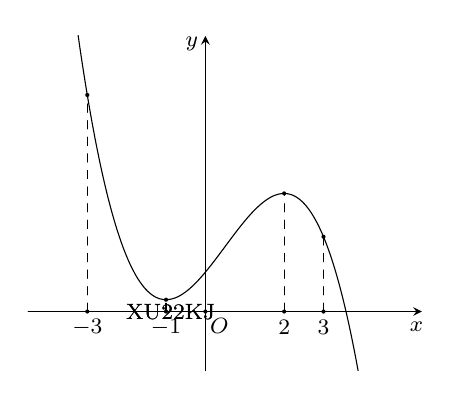
\begin{tikzpicture}[scale=0.5, font=\footnotesize, line join=round, line cap=round, >=stealth]
    %hidden: VM005
				\def \xmin{-4.5}\def \xmax{5.5}\def \ymin{-1.5}\def \ymax{7} 
				\draw[->] (\xmin,0)--(\xmax,0) node[shift=(-110:0.2)] {$x$};
				\draw[->] (0,\ymin)--(0,\ymax) node[shift=(-150:0.2)] {$y$};
				\fill (0,0) node{\href{XU22KJ}{\tiny \phantom{XU22KJ}}} circle(1pt) node[shift=(-45:0.25)]{$O$};
				\clip (\xmin,\ymin) rectangle (\xmax,\ymax);
				\draw[smooth,samples=100,domain=\xmin:\xmax] plot({\x}, {-0.2*\x*\x*\x + 0.3*\x*\x + 1.2*\x + 1});
				\draw[dashed] (-3,0) -- (-3, 5.5);
				\draw[dashed] (-1,0) -- (-1, 0.3);
				\draw[dashed] (2,0)  -- (2, 3.0);
				\draw[dashed] (3,0)  -- (3, 1.9);
				\fill (-3,0) circle (1.5pt) node[shift=(-90:0.2)] {$-3$};
				\fill (-1,0) circle (1.5pt) node[shift=(-90:0.2)] {$-1$};
				\fill (2,0)  circle (1.5pt) node[shift=(-90:0.2)] {$2$};
				\fill (3,0)  circle (1.5pt) node[shift=(-90:0.2)] {$3$};
				\fill (-3, 5.5) circle (1.5pt);
				\fill (-1, 0.3) circle (1.5pt);
				\fill (0, 0)  circle (1.5pt);
				\fill (2, 3.0)  circle (1.5pt);
				\fill (3, 1.9)  circle (1.5pt);
    \node at (0,0){\href{XU22KJ}{\tiny \phantom{XU22KJ}}};
			\end{tikzpicture}
			}
	\loigiai{
		Dựa vào đồ thị hàm số, ta thấy điểm của tọa độ $\left(-3;f(-3)\right)$ cao nhất so với các điểm còn lại trên đoạn $[-3;3]$.\\
		Do đó, giá trị lớn nhất của hàm số đã cho trên đoạn $[-3;3]$ bằng $f(-3)$.
	}
\end{ex}

\Closesolutionfile{ans}
\cauds
\Opensolutionfile{ans}[ans/ans\currfilebase-Phan-II]
\begin{ex}%[Dự án 1QI8CW-VN-MT-15]%[2-KS-30-CumDakLak-L1-2026,VM036,TV013]%[2D1V5-7]
	Cho hàm số $y=f(x)=ax^3+bx^2+cx+d$ có bảng biến thiên như sau:
	\begin{center}
		\begin{tikzpicture}
    %hidden: VM005
			\tkzTabInit[nocadre=true, lgt=1, espcl=3, deltacl=0.5]
			{$x$ /.7, $y'$ /.7, $y$/2} 
			{$-\infty$, $1$, $3$, $+\infty$}
			\tkzTabLine{ ,-,$0$,+,$0$,-, }
			\tkzTabVar{+/$+\infty$, -/$2$, +/$4$, -/$-\infty$}
    \node at (T11){\href{1QI8CW}{\tiny \phantom{1QI8CW}}};
		\end{tikzpicture}
	\end{center}
	\choiceTF
		{\True Hàm số có hệ số $a<0$}
		{$f'(x)=0$ tại các giá trị $x=2$, $x=4$}
		{\True Đồ thị hàm số đi qua hai điểm $(1;2)$, $(3;4)$}
		{Giá trị nhỏ nhất của hàm số trên $[2;4]$ bằng $\dfrac{7}{2}$}
	\loigiai{
		\begin{itemchoice}
			\itemch 
			Từ bảng biến thiên, ta có $\lim\limits_{x\to+\infty} f(x)=-\infty$. Suy ra hệ số $a<0$.
			\itemch 
			Dựa vào bảng biến thiên, ta có $f'(x)=0 \Leftrightarrow \hoac{&x=1\\ &x=3.}$
			\itemch 
			Đồ thị hàm số có hai điểm cực trị là $A(1;2)$ và $B(3;4)$.\\
			Suy ra đồ thị đi qua hai điểm $(1;2)$ và $(3;4)$.
			\itemch 
			Ta có $y'=f'(x)=3ax^2+2bx+c$.\\
			Vì đồ thị hàm số có hai điểm cực trị là $A(1;2)$ và $B(3;4)$ nên ta có
			\[\heva{&f'(1)=0\\&f(1)=2\\&f'(3)=0\\&f(3)=4}\Leftrightarrow \heva{&3a+2b+c=0\\&a+b+c+d=2\\&27a+6b+c=0\\&27a+9b+3c+d= 4} \Leftrightarrow \heva{&a=-\dfrac{1}{2}\\&b=3\\&c=-\dfrac{9}{2}\\&d=4.}\]
			Suy ra $f(x)=-\dfrac{1}{2}x^3+3x^2-\dfrac{9}{2}x+4$.\\
			Ta có $f(2)=3$, $f(3)=4$, $f(4)=2$.\\
			Suy ra $\min\limits_{[2;4]} f(x)=2$.
		\end{itemchoice}
	}
\end{ex}

\begin{ex}%[Dự án C571KW-VN-MT-15]%[2-KS-30-CumDakLak-L1-2026,VM036,TV013]%[2D4V1-6]
	Ở nhiệt độ $37^\circ\mathrm{C}$, một phản ứng hóa học từ chất đầu $A$, chuyển hóa thành chất sản phẩm $B$ theo phương trình $A \to B$. Giả sử $y(x)$ là nồng độ chất $A$ (đơn vị mol/L) tại thời điểm $x$ (giây), $y(x)>0$ với $x\ge 0$, thỏa mãn hệ thức $y'(x)=-7 \cdot 10^{-4}y(x)$ với $x\ge 0$. Biết rằng tại $x=0$, nồng độ (đầu) của $A$ là $0{,}05$\,mol/L. Xét hàm số $f(x)=\ln y(x)$ với $x\ge 0$. Khi đó, ta có
	\choiceTF
		{\True $f'(x)=-7\cdot 10^{-4}$}
		{\True $f(x)=-7\cdot 10^{-4}x+\ln(0{,}05)$}
		{$y(30)-y(15)=-6\cdot 10^{-4}$}
		{\True Nồng độ trung bình của chất $A$ từ thời điểm $15$ giây đến thời điểm $30$ giây bằng $0{,}05$ (\textit{kết quả đã làm tròn đến hàng phần trăm})}
	\loigiai{
		\begin{itemchoice}
			\itemch 
			Ta có $f'(x)=\left[\ln y(x)\right]'=\dfrac{y'(x)}{y(x)}=-7\cdot 10^{-4}$.
			\itemch 
			Ta có $f(x)=\displaystyle\int f'(x)\mathrm{\,d}x=\displaystyle\int\left(-7\cdot 10^{-4}\right)\mathrm{\,d}x=-7\cdot 10^{-4}x+C$.\\
			Theo giả thiết $y(0)=0{,}05$ nên $f(0)=\ln y(0)=\ln(0{,}05)$.\\ 
			Khi đó $C=\ln(0{,}05)$.\\
			Vậy $f(x)=-7\cdot 10^{-4}x+\ln(0{,}05)$.
			\itemch 
			Từ $f(x)=\ln y(x)$, suy ra $y(x)=\mathrm{e}^{f(x)}=\mathrm{e}^{-7\cdot 10^{-4}x+\ln(0{,}05)}=\dfrac{1}{20}\mathrm{e}^{-7\cdot 10^{-4}x}$.\\
			Do đó $y(30)-y(15)=\dfrac{1}{20}\left(\mathrm{e}^{-7\cdot 10^{-4}\cdot 30}-\mathrm{e}^{-7\cdot 10^{-4}\cdot 15}\right)\approx -5{,}2\cdot 10^{-4}$.
			\itemch 
			Nồng độ trung bình của chất $A$ từ thời điểm $15$ giây đến thời điểm $30$ giây là
			\allowdisplaybreaks
			\begin{align*}
				\dfrac{1}{30-15}\displaystyle\int\limits_{15}^{30} y(x)\mathrm{\,d}x &= \dfrac{1}{15}\displaystyle\int\limits_{15}^{30} 0{,}05\mathrm{e}^{-7 \cdot 10^{-4}x}\mathrm{\,d}x \\
				&=\dfrac{1}{15} \left(0{,}05 \cdot \dfrac{\mathrm{e}^{-7\cdot 10^{-4}x}}{-7\cdot 10^{-4}}\right)\Bigg|_{15}^{30} \\
				&=-\dfrac{1}{15}\cdot \dfrac{500}{7} \left(\mathrm{e}^{-7 \cdot 10^{-4}x}\right)\Bigg|_{15}^{30} \\
				&=-\dfrac{100}{21} \left(\mathrm{e}^{-0{,}021}-\mathrm{e}^{-0{,}0105}\right)\approx 0{,}05\text{ (mol/L)}.
			\end{align*}
		\end{itemchoice}
	}
\end{ex}

\begin{ex}%[Dự án 20BVDK-VN-MT-15]%[2-KS-30-CumDakLak-L1-2026,VM036,TV013]%[2D6V2-4]
	Trước kỳ thi tốt nghiệp THPT năm 2026, trường THPT X khảo sát $560$ học sinh về việc đăng ký xét tuyển đại học bằng học bạ. Kết quả thống kê như sau: có $392$ học sinh trả lời \lq\lq sẽ xét học bạ\rq\rq. Qua theo dõi thực tế, tỉ lệ học sinh thực sự xét tuyển học bạ tương ứng với những cách trả lời \lq\lq sẽ xét học bạ\rq\rq\ và \lq\lq không xét học bạ\rq\rq\ lần lượt là $80\%$ và $10\%$. Gọi $A$ là biến cố: \lq\lq Học sinh thực sự xét học bạ\rq\rq\ và $B$ là biến cố: \lq\lq Học sinh trả lời sẽ xét học bạ\rq\rq.
	\choiceTF
		{\True Xác suất $\mathrm{P}(B)=0{,}7$ và $\mathrm{P}\left(\overline{B}\right)=0{,}3$}
		{Xác suất có điều kiện $\mathrm{P}(A\mid\overline{B}) = 0{,}2$}
		{\True Xác suất $\mathrm{P}(A) = 0{,}59$}
		{Trong số những học sinh thực sự xét tuyển bằng học bạ, xác suất học sinh đó trả lời \lq\lq sẽ xét học bạ\rq\rq\ nhỏ hơn $90\%$}
	\loigiai{
		Xác suất học sinh trả lời sẽ xét học bạ là $\mathrm{P}(B)=\dfrac{392}{560}=0{,}7$. Suy ra $\mathrm{P}\left(\overline{B}\right)=1-0{,}7=0{,}3$.\\
		Theo giả thiết, ta có xác suất có điều kiện $\mathrm{P}(A\mid B)=80\%=0{,}8$ và $\mathrm{P}\left(A\mid\overline{B}\right)=10\%=0{,}1$.\\
		Sơ đồ cây biểu diễn các xác suất như sau:
		\begin{center}
			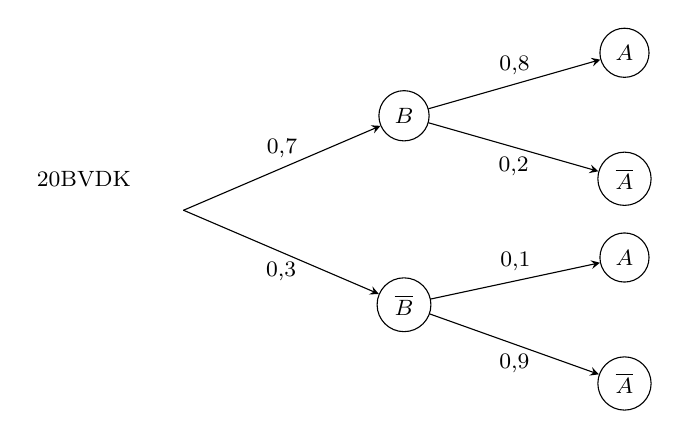
\begin{tikzpicture}[scale=.4, font=\footnotesize, line join=round, line cap=round, >=stealth]
    %hidden: VM005
				\coordinate (O) at (2,-1);
				\begin{scope}[every node/.style={circle,draw=black}]
					\node (A) at (9,2) {$B$};
					\node (B) at (9,-4) {$\overline{B}$};
					\node (C) at (16,4) {$A$};
					\node (D) at (16,0) {$\overline{A}$};
					\node (E) at (16,-2.5) {$A$};
					\node (F) at (16,-6.5) {$\overline{A}$}; 
				\end{scope}
				\draw[->] (O)--(A)node[midway,above]{$0{,}7$};
				\draw[->] (A)--(C)node[midway,above]{$0{,}8$};
				\draw[->] (A)--(D)node[midway,below]{$0{,}2$};
				\draw[->] (O)--(B)node[midway,below]{$0{,}3$};
				\draw[->] (B)--(E)node[midway,above]{$0{,}1$};
				\draw[->] (B)--(F)node[midway,below]{$0{,}9$};
    \node at (0,0){\href{20BVDK}{\tiny \phantom{20BVDK}}};
			\end{tikzpicture}
		\end{center}
		\begin{itemchoice}
			\itemch 
			Ta có $\mathrm{P}(B)=\dfrac{392}{560}=0{,}7$; $\mathrm{P}\left(\overline{B}\right)=1-\mathrm{P}(B)= 0{,}3$.
			\itemch 
			Theo giả thiết, tỉ lệ học sinh thực sự xét học bạ trong số những học sinh trả lời không xét là $10\%$ nên $\mathrm{P}\left(A\mid \overline{B}\right)= 0{,}1$.
			\itemch 
			Áp dụng công thức xác suất toàn phần, ta có
			\[\mathrm{P}(A)=\mathrm{P}(B)\cdot\mathrm{P}(A\mid B)+\mathrm{P}\left(\overline{B}\right)\cdot\mathrm{P}\left(A\mid\overline{B}\right)=0{,}7\cdot 0{,}8+0{,}3\cdot 0{,}1=0{,}56+0{,}03=0{,}59.\]
			\itemch 
			Áp dụng công thức Bayes, ta có
			\[\mathrm{P}(B\mid A)=\dfrac{\mathrm{P}(A\cap B)}{\mathrm{P}(A)}=\dfrac{\mathrm{P}(B)\cdot \mathrm{P}(A\mid B)}{\mathrm{P}(A)}=\dfrac{0{,}7\cdot 0{,}8}{0{,}59}=\dfrac{56}{59}\approx 94{,}9\%>90\%.\]
		\end{itemchoice}
	}
\end{ex}

\begin{ex}%[Dự án 2ME9T6-VN-MT-15]%[2-KS-30-CumDakLak-L1-2026,VM036,TV013]%[2H5V2-8]
	Trong không gian $Oxyz$ (đơn vị trên mỗi trục là km), một tàu đánh cá gặp nạn đang phát tín hiệu cấp cứu tại vị trí $T(1;-2;1)$, tín hiệu này có bán kính phủ sóng tối đa là $9$\,km. Một trực thăng cứu hộ đang bay từ vị trí $P(10;10;13)$ theo hướng vectơ $\overrightarrow{u}=(-3; -4;-4)$ với tốc độ không đổi $150$\,km/h.
	\choiceTF
		{\True Phương trình đường bay của trực thăng cứu hộ là $\dfrac{x-10}{-3}=\dfrac{y-10}{-4}=\dfrac{z-13}{-4}$}
		{\True Phương trình vùng phủ sóng cứu nạn là mặt cầu $x^2+y^2+z^2-2x+4y-2z-75=0$}
		{Vị trí đầu tiên trực thăng nhận được tín hiệu cứu nạn là $(4;2;5)$}
		{Kể từ khi nhận được tín hiệu cứu nạn, trực thăng cần đúng $6$ phút để bay đến vị trí gần tàu gặp nạn nhất (\textit{giả sử tốc độ bay của trực thăng cứu nạn không thay đổi})}
	\loigiai{
		\begin{center}
			\begin{tikzpicture}[scale=1, font=\footnotesize, line join=round, line cap=round, >=stealth]
    %hidden: VM005
				\def\R{2.5}
				\def\Ry{0.75}
				\coordinate (T) at (0,0);
				\draw[dashed] (\R,0) arc (0:180:{\R} and {\Ry});
				\draw (-\R,0) arc (180:360:{\R} and {\Ry});
				\draw (0,0) circle (\R);
				\coordinate (P) at (5,3.5);
				\coordinate (M) at ($(T)!2.5cm!(P)$);
				\coordinate (N) at ($(T)!-2.5cm!(P)$);
				\coordinate (P_end) at ($(T)!-4cm!(P)$);
				\draw (P) -- (M);
				\draw[dashed] (M) -- (N);
				\draw[->] (N) -- (P_end) node[below left] {Hướng bay};
				\draw[->] (P) -- ($(P)!0.2!(M)$) node[above left] {$\overrightarrow{u}$};
				\fill (T) circle (1pt) node[shift=(-15:0.9)] {$T (1; -2; 1)$};
				\fill (P) circle (1pt) node[above right] {$P (10; 10; 13)$};
				\fill (M) circle (1pt) node[right=2pt] {$M$};
				\draw[<-] (M) -- ++(-0.2,0.8) node[above,align=right] {Bắt đầu nhận\\tín hiệu};
				\draw[dashed] (T) -- (-\R,0) node[midway,above] {$R=9$};
    \node at (0,0){\href{2ME9T6}{\tiny \phantom{2ME9T6}}};
			\end{tikzpicture}
		\end{center}
		\begin{itemchoice}
			\itemch 
			Đường bay của trực thăng là đường thẳng đi qua $P(10;10;13)$ và nhận $\overrightarrow{u}=(-3;-4;-4)$ làm vectơ chỉ phương nên có phương trình chính tắc là $\dfrac{x-10}{-3}=\dfrac{y-10}{-4}=\dfrac{z-13}{-4}$.
			\itemch 
			Vùng phủ sóng là mặt cầu tâm $T(1;-2;1)$, bán kính $R=9$ có phương trình là
			\allowdisplaybreaks
			\begin{eqnarray*}
				&&(x-1)^2+(y+2)^2+(z-1)^2=81\\
				&\Leftrightarrow&x^2+y^2+z^2-2x+4y-2z-75=0.
			\end{eqnarray*}
			\itemch 
			Ta thấy $M(4;2;5)$ nằm trên đường bay $\dfrac{x-10}{-3}=\dfrac{y-10}{-4}=\dfrac{z-13}{-4}$.\\
			Mặt khác $TM=\sqrt{(4-1)^2+(2+2)^2+(5-1)^2}=\sqrt{41}\approx 6{,}4$\,km.\\ 
			Vì $TM<R$ nên $M(4;2;5)$ đã nằm sâu trong vùng phủ sóng (trực thăng đã nhận được tín hiệu từ trước khi bay đến $M$).\\ 
			Do đó $M$ không phải điểm đầu tiên nhận tín hiệu.
			\itemch 
			Phương trình tham số của đường bay là $\heva{&x=10-3t\\&y=10-4t\\&z=13-4t}$ $(t\ge 0)$.\\
			Khoảng cách từ vị trí $A(10-3t; 10-4t;13-4t)$ của trực thăng đến vị trí $T (1; -2; 1)$ của tàu là
			\[\mathrm{d}=AT=\sqrt{(3t-9)^2+(4t-12)^2+(4t-12)^2}=\sqrt{41(t-3)^2}=|t-3|\sqrt{41}.\]
			Khoảng cách này đạt giá trị nhỏ nhất bằng $0$ khi $t=3$. Nghĩa là đường bay của trực thăng đi ngang qua chính xác vị trí tàu $T(1;-2;1)$.\\
			Khoảng cách từ điểm bắt đầu nhận tín hiệu (rìa vùng phủ sóng) đến tàu $T$ chính là bán kính $R=9$\,km.\\
			Vậy thời gian để trực thăng bay quãng đường $9$\,km với tốc độ $150$\,km/h là
			\[t_{\text{bay}}=\dfrac{9}{150}=0{,}06\text{ (giờ)}= 3{,}6\text{ (phút)}.\]
		\end{itemchoice}
	}
\end{ex}

\Closesolutionfile{ans}
\caukq
\Opensolutionfile{ans}[ans/ans\currfilebase-Phan-III]
\begin{ex}%[Dự án 5VJTOD-VN-MT-15]%[2-KS-30-CumDakLak-L1-2026, VM006]%[1D2V3-8]
	Anh An vừa tốt nghiệp đại học và được nhận vào làm việc tại một công ty với một trong hai phương án lương như sau:
	\begin{itemize}
		\item Phương án $1$: lương khởi điểm $10$ triệu đồng một tháng, cứ sau tròn $3$ năm thì tăng lương mỗi tháng $6$ triệu đồng so với mỗi tháng của $3$ năm trước đó.
		\item Phương án $2$: lương khởi điểm $10$ triệu đồng một tháng, cứ sau tròn $3$ năm thì tăng lương mỗi tháng $40\%$, so với mỗi tháng của $3$ năm trước đó.
	\end{itemize}
	Nếu anh An kí hợp đồng làm việc $20$ năm thì sau $20$ năm đi làm, tổng tiền lương anh nhận được theo phương án $2$ nhiều hơn phương án $1$ bao nhiêu triệu đồng (\textit{làm tròn kết quả đến hàng đơn vị})?
	\par
	\shortans{$1\,180$}
	\loigiai{
		Ta có $20=3\cdot6+2$; $3$ năm $=36$ tháng và $2$ năm $=24$ tháng.\\
		Số tiền nhận được sau $20$ năm đi làm nếu kí hợp đồng theo phương án $1$ là
		\[
		T_1=36 \cdot (10+16+22+28+34+40)+24\cdot 46=6\,504~\text{(triệu đồng)}.
		\]
		Số tiền nhận được sau $20$ năm đi làm nếu kí hợp đồng theo phương án $2$ là
		\begin{align*} 
			T_2&=36\cdot\left(10+10\cdot1{,}4+10\cdot1{,}4^2+10\cdot1{,}4^3+10\cdot1{,}4^4+10\cdot1{,}4^5\right)+24\cdot10\cdot1{,}4^6  \\ 
			&=36\cdot10\left(1+1{,}4+1{,}4^2+1{,}4^3+1{,}4^4+1{,}4^5\right)+24\cdot10\cdot1{,}4^6  \\ 
			&=36\cdot10\cdot\dfrac{1-1{,}4^6}{1-1{,}4}+24\cdot10\cdot1{,}4^6  \\ 
			&=\dfrac{24\,011\,472}{3\,125}~\text{(triệu đồng)}. 
		\end{align*}
		Suy ra tổng tiền lương anh nhận được theo phương án $2$ nhiều hơn phương án $1$ là
		\[
		\Delta T=T_2-T_1=\dfrac{24\,011\,472}{3\,125}-6\,504\approx 1\,180~\text{(triệu đồng)}. 
		\]
	}
\end{ex}

\begin{ex}%[Dự án 20YA21-VN-MT-15]%[2-KS-30-CumDakLak-L1-2026, VM006]%[2H5V2-6]
	Trong không gian $Oxyz$, cho hai điểm $A(-1;4;4)$, $B(-4;6;5)$ và đường thẳng\break $d \colon \dfrac{x-2}{2} = \dfrac{y-3}{3} = \dfrac{z+4}{-5}$. Một điểm $C$ thay đổi trên $d$ có giá trị nhỏ nhất của diện tích $ABC$ bằng $\sqrt{a}$. Giá trị $\dfrac{a}{6}$ bằng bao nhiêu?
	\par
	\shortans{$7$}
	\loigiai{
		Ta có $\overrightarrow{AB}=(-3;2;1)\Rightarrow AB=\sqrt{14}$.\\
		Đường thẳng $AB$ đi qua điểm $A(-1;4;4)$ và nhận $\overrightarrow{AB}=(-3;2;1)$ làm một vectơ chỉ phương nên có phương trình tham số là
		$\heva{&x=-1-3t \\&y = 4+2t \\&z=4+t.}$\\
		Gọi $P(-1-3p; 4+2p; 4+p)\in AB$ và $Q(2+2q;3+3q;-4-5q) \in d$.\\
		Ta có $\overrightarrow{PQ}= (2q+3p+3;3q-2p-1;-5q-p-8)$.\\
		Giả sử $PQ$ là đoạn vuông góc chung của $AB$ và $d$. Khi đó, ta có
		\allowdisplaybreaks
		\begin{eqnarray*} 
			&&\heva{&\overrightarrow{PQ} \perp \overrightarrow{u}_d \\&\overrightarrow{PQ} \perp \overrightarrow{AB}}  \\ 
			&\Leftrightarrow&\heva{&2(2q+3p+3)+3(3q-2p-1)-5(-5q-p-8)=0 \\&-3(2q+3p+3)+2(3q-2p-1)+1(-5q-p-8)=0}   \\ 
			&\Leftrightarrow&\heva{&38q+5p=-43 \\&-5q-14p=19}   \\ 
			&\Leftrightarrow&\heva{&q=-1 \\&p=-1.}
		\end{eqnarray*}
		Suy ra $ P(2;2;3)$, $Q(0;0;1)$ và $PQ =\sqrt{2^2+2^2+2^2}= 2\sqrt{3}$.\\
		Do đó, khoảng cách nhỏ nhất từ $C$ đến đường thẳng $AB$ là $\mathrm{d}(d, AB) = PQ = 2\sqrt{3}$.\\
		Suy ra diện tích nhỏ nhất của tam giác $ABC$ là 
		\[
		S_{\triangle ABC}=\dfrac{1}{2}\cdot AB\cdot PQ = \dfrac{1}{2}\cdot\sqrt{14}\cdot 2\sqrt{3}=\sqrt{42}.
		\]
		Vậy $a=42$ và $\dfrac{a}{6}=\dfrac{42}{6}=7$.
	}
\end{ex}

\begin{ex}%[Dự án 38V4OH-VN-MT-15]%[2-KS-30-CumDakLak-L1-2026, VM006]%[1H8V7-2]
	Cho khối lăng trụ $ABC.A'B'C'$ có đáy là tam giác đều cạnh $a$, hình chiếu vuông góc của điểm $A'$ lên mặt phẳng $(ABC)$ trùng với trọng tâm của tam giác $ABC$. Biết khoảng cách giữa hai đường thẳng $AA'$ và $BC$ bằng $\dfrac{a\sqrt{3}}{4}$, thể tích khối chóp $A'.ABC$ bằng $\dfrac{a^3 \sqrt{m}}{n}$ ($\,m, n \in \mathbb{N}^*$ và $m$ là số nguyên tố). Tính $m+n$.
	\par
	\shortans{$39$}
	\loigiai{
		\begin{center}
			\begin{tikzpicture}[scale=1, font=\footnotesize, line join=round, line cap=round, >=stealth]
    %hidden: VM005
				\coordinate (A) at (0,0);
				\coordinate (B) at (2.1,-1.8);
				\coordinate (C) at (5,0);
				\path ($(B)!0.5!(C)$) coordinate (K);
				\path ($(A)!2/3!(K)$) coordinate (O);
				\coordinate (A') at ($(O)+(0,4)$);
				\path ($(A')+1*(B)-1*(A)$) coordinate (B');
				\path ($(A')+1*(C)-1*(A)$) coordinate (C');
				\path ($(A')!0.4!(A)$) coordinate (I);
				\path ($(A)!2/3!(I)$) coordinate (H);
				\draw (A)--(B)--(C) (A')--(B')--(C')--cycle (A)--(A') (B)--(B') (C)--(C');
				\draw[dashed] (A)--(C) (A)--(K) (A')--(O) (A')--(K)--(I) (O)--(H);
				\foreach \x/\g in{A/180,B/-90,C/0,K/-30,O/-90,A'/160,B'/-60,C'/0,I/120,H/120}\fill(\x) circle (1pt)+(\g:.3) node{$\x$};
				\foreach \x/\y/\z in {K/I/A',O/H/A',A/K/B}{
				\path pic[draw,angle radius=5pt]{right angle= \x--\y--\z};
			}
    \node at (0,0){\href{38V4OH}{\tiny \phantom{38V4OH}}};
			\end{tikzpicture}
		\end{center}
		Gọi $K$ là trung điểm của $BC$ và $O$ là trọng tâm của $\triangle ABC$.\\
		Kẻ $KI \perp AA'$ tại $I$ và $OH \perp AA'$ tại $H$. \\
		Ta có $\heva{&BC \perp AK \ \text{ (do $\triangle ABC$ đều)}\\ &BC \perp A'O \ \text{ (do $A'O\perp (ABC)$)}\\ &AK \cap A'O=O}$, suy ra $BC \perp \left(A'AK\right)$.\\
		Mà $IK \subset (A'AK)$ nên $BC \perp IK$. \\
		Ta có $\heva{&IK \perp AA' \text{ tại } I \\&IK \perp BC \text{ tại } K}$ nên $IK$ là đoạn vuông góc chung của hai đường thẳng $AA'$ và $BC$.\\
		Suy ra $IK =\mathrm{d}\left(AA', BC\right)= \dfrac{a\sqrt{3}}{4}$. \\
		Ta có $OH \parallel IK \Rightarrow \dfrac{OH}{IK}=\dfrac{AO}{AK}=\dfrac{2}{3}\Rightarrow OH=\dfrac{2}{3}IK=\dfrac{a\sqrt{3}}{6}$. \\
		Lại có $AO=\dfrac{2}{3}AK=\dfrac{2}{3}\cdot\dfrac{a\sqrt{3}}{2}= \dfrac{a\sqrt{3}}{3}$. \\
		Xét tam giác $A'OA$ vuông tại $O$, có $OH$ là đường cao nên
		\[
		\dfrac{1}{OH^2}=\dfrac{1}{OA^2}+\dfrac{1}{OA'^2}\Rightarrow OA'=\dfrac{OA\cdot OH}{\sqrt{OA^2-OH^2}}=\dfrac{a}{3}.
		\]
		Suy ra $V_{A'.ABC} = \dfrac{1}{3} \cdot OA' \cdot S_{\triangle ABC} = \dfrac{1}{3} \cdot \dfrac{a}{3} \cdot \dfrac{a^2\sqrt{3}}{4} = \dfrac{a^3\sqrt{3}}{36}$.\\ 
		Vậy $\heva{&m=3 \\&n=36}$ và $m+n=39$.
	}
\end{ex}

\begin{ex}%[Dự án 20WR66-VN-MT-15]%[2-KS-30-CumDakLak-L1-2026, TV035]%[2D4V3-2]
	Để chuẩn bị cho lễ kỷ niệm $20$ năm ngày ra trường, ban tổ chức quyết định đặt hàng một đơn vị thủ công mỹ nghệ để chế tác các huy hiệu cài áo đặc biệt như hình vẽ sau:
	\begin{center}
		\begin{tikzpicture}[scale=1, font=\footnotesize, line join=round, line cap=round, >=stealth]
    %hidden: VM005
			\def\xmin{-0.5}\def\xmax{6}\def\ymin{-1}\def\ymax{6}
			\tikzset{declare function={f(\x) = -1/6*\x*\x + 5/6*\x;}}
			\coordinate (O) at (0,0);
			\coordinate (A) at (5,0);
			\coordinate (B) at (5,5);
			\coordinate (C) at (0,5);
			\coordinate (M) at (2,1);
			\coordinate (M1) at (2,0);
			\coordinate (M2) at (0,1);
			\draw[dashed, |<->|] ($(A)+(0.2,0)$) -- ($(B)+(0.2,0)$) node[midway,right]{$20$\,mm};
			\draw[dashed] (0,1) -- (2,1) node[midway,above]{$8$\,mm} -- (2,0) node[midway,right]{$4$\,mm} ;
			\fill[blue!50] (C) -- (B) -- (A) 
				-- plot[domain=5:2, smooth, samples=50] (\x, {f(\x)})
				arc ({asin(-0.6)}:90:2.5) -- cycle;
			\draw (O) rectangle (B);
			\draw (M) arc ({asin(-0.6)}:90:2.5);
			\draw[smooth, samples=100, domain=2:5] plot (\x, {f(\x)});
			\foreach \x/\pos in {O/-135, A/-90, B/90, C/135} \fill (\x) circle(1pt) node[{shift=(\pos:0.25)}]{$\x$}; 
			\fill (M) circle(1pt) node[{shift=(-135:0.3)}]{$M$}; 
			\foreach \x in {M1, M2} \fill (\x) circle(1pt);
    \node at (0,0){\href{20WR66}{\tiny \phantom{20WR66}}};
		\end{tikzpicture}
	\end{center}
	Huy hiệu được thiết kế trên một phôi bạc hình vuông $OABC$ có cạnh bằng $20$\,mm. Theo bản vẽ kỹ thuật từ các nghệ nhân, cấu trúc của huy hiệu được phân chia như sau: lấy một điểm $M$ được xác định bên trong phôi bạc sao cho khoảng cách từ $M$ đến cạnh dưới $OA$ là $4$\,mm và cách cạnh bên trái $OC$ là $8$\,mm, cạnh vòm là một nửa cung tròn đi qua ba điểm $O$, $M$, $C$; đường lượn là một phần của parabol đi qua ba điểm $O$, $M$, $A$. Phần tô đậm trong bản vẽ sẽ được phủ men sứ màu xanh lam. Các phần tử còn lại sẽ được giữ nguyên màu bạc để khắc tên trường và niên khóa. Tính diện tích phần tô đậm trong bản vẽ được phủ men sứ màu xanh {\it (kết quả làm tròn đến hàng đơn vị theo đơn vị mm$^2$).}
	\par \shortans{$197$}
	\loigiai{
		Chọn hệ trục tọa độ $Oxy$ như hình vẽ sau:
		\begin{center}
			\begin{tikzpicture}[scale=1, font=\footnotesize, line join=round, line cap=round, >=stealth]
    %hidden: VM005
				\def\xmin{-0.5}\def\xmax{6}\def\ymin{-1}\def\ymax{6}
				\draw[->] (\xmin-0.2,0)--(\xmax+0.2,0) node[below]{$x$};
				\draw[->] (0,\ymin-0.2)--(0,\ymax+0.2) node[right]{$y$};
				\tikzset{declare function={f(\x) = -1/6*\x*\x + 5/6*\x;}}
				\coordinate (O) at (0,0);
				\coordinate (A) at (5,0);
				\coordinate (B) at (5,5);
				\coordinate (C) at (0,5);
				\coordinate (M) at (2,1);
				\draw[dashed] (0,1) -- (2,1) -- (2,0);
				\fill (0,1) circle (1pt) node[left]{$4$};
				\fill (0,5) circle (1pt) node[left]{$20$};
				\fill (2,0) circle (1pt) node[below]{$8$};
				\fill (5,0) circle (1pt) node[below]{$20$};
				\fill[blue!40] (C) -- (B) -- (A) 
					-- plot[domain=5:2, smooth, samples=50] (\x, {f(\x)})
					arc ({asin(-0.6)}:90:2.5) -- cycle;
				\draw (O) rectangle (B);
				\draw (C) arc (90:-90:2.5);
				\draw[smooth, samples=100, domain=0:5] plot (\x, {f(\x)});
				\foreach \x/\pos in {O/-135, A/45, B/30, C/45, M/135} \fill (\x) circle(1pt) node[{shift=(\pos:0.25)}]{$\x$}; 
    \node at (0,0){\href{20WR66}{\tiny \phantom{20WR66}}};
			\end{tikzpicture}
		\end{center}
		Theo giả thiết, ta có $A(20;0)$, $C(0;20)$ và $M(8;4)$. \\
		Đường tròn qua ba điểm $O$, $M$, $C$ có tâm $(0;10)$, bán kính $R=10$ có phương trình là 
		\[
		x^2 + (y-10)^2 =100. 
		\]
		Phần đồ thị phía dưới chứa cung $OM$ có phương trình là $y=-\sqrt{100-x^2} +10$. \\
		Diện tích nửa đường tròn đường kính $OC$ là $S_1 = \dfrac{1}{2} \pi R^2 = 50\pi$ (mm$^2$). \\
		Parabol đi qua hai điểm $O(0;0)$ và $A(20;0)$ nên có phương trình là $y=a x (x-20)$. \\
		Lại có điểm $M(8;4)$ thuộc parabol nên $4=a \cdot 8 \cdot (8-20) \Rightarrow a= - \dfrac{1}{24}$. \\
		Vậy phương trình của parabol là $y=-\dfrac{1}{24} x (x-20) = -\dfrac{1}{24} x^2 + \dfrac{5}{6}x$. \\
		Diện tích phần tô màu là 
		\[
		S=20^2 - 50\pi - \int\limits_{0}^{8} \left(-\sqrt{100-x^2} +10\right) \mathrm{d}x - \int\limits_{8}^{20} \left(- \dfrac{1}{24} x^2 + \dfrac{5}{6} x\right) \mathrm{d}x \approx 197\, (\text{mm}^2). 
		\]
	}
\end{ex}

\begin{ex}%[Dự án 2Q4PKD-VN-MT-15]%[2-KS-30-CumDakLak-L1-2026, TV035]%[1D9V2-4]
	Chọn ngẫu nhiên $3$ trong số $24$ đỉnh của một đa giác đều $24$ cạnh. Gọi $P$ là xác suất để ba đỉnh được chọn là ba đỉnh của một tam giác cân hoặc một tam giác vuông. Biết $P=\dfrac{a}{b}$ với $a$, $b \in \mathbb{N}^{*}$ và $\dfrac{a}{b}$ là phân số tối giản. Tính $2a+b$. 
	\par \shortans{$375$}
	\loigiai{
		Số phần tử của không gian mẫu là $n (\Omega) = \mathrm{C}^{3}_{24} = 2\,024$. \\
		Gọi các biến cố sau:
		\begin{itemize}
			\item $A$ là biến cố \lq\lq Ba đỉnh được chọn là ba đỉnh của một tam giác cân\rq\rq;
			\item $B$ là biến cố \lq\lq Ba đỉnh được chọn là ba đỉnh của một tam giác vuông\rq\rq.
		\end{itemize}
		Suy ra 
		\begin{itemize}
			\item $AB$ là biến cố \lq\lq Ba đỉnh được chọn là ba đỉnh của một tam giác vuông cân\rq\rq;
			\item $A \cup B$ là biến cố \lq\lq Ba đỉnh được chọn là ba đỉnh của một tam giác cân hoặc một tam giác vuông\rq\rq.
		\end{itemize}
		Gọi $(O)$ là đường tròn ngoại tiếp đa giác đều ban đầu. Khi đó, ta có các trường hợp sau:
		\begin{itemize}
			\item Mỗi tam giác vuông được lập thành từ ba đỉnh của đa giác thì có cạnh huyền là đường kính của đường tròn $(O)$. \\
			Ta có $12$ cách chọn đường kính. \\
			Với mỗi cách chọn đường kính, ta có $22$ cách chọn đỉnh góc vuông. \\
			Do đó, số tam giác vuông lập từ $3$ đỉnh của đa giác là $12 \cdot 22 = 264$. 
			\item Mỗi tam giác cân có ba đỉnh là ba đỉnh của đa giác thì đường cao của tam giác cân đó phải là đường kính của đường tròn $(O)$. \\
			Với mỗi đỉnh của đa giác, ta có $10$ cách tạo ra các tam giác cân (không đều). \\
			Do đó, số tam giác cân thỏa mãn yêu cầu là $10 \cdot 24 =240$. 
			\item Số tam giác đều có ba đỉnh là ba đỉnh của đa giác là $24 : 3 = 8$. 
			\item Với mỗi cách chọn đường kính, ta có hai cách chọn đỉnh góc vuông để tạo thành tam giác vuông cân. \\
			Do đó, số tam giác vuông cân là $12 \cdot 2 = 24$. 
		\end{itemize}
		Suy ra xác suất cần tìm là
		\[
		P=\mathrm{P} (A \cup B) = \mathrm{P} (A) + \mathrm{P} (B) - \mathrm{P} (AB) =\dfrac{248}{2\,024} + \dfrac{264}{2\,024} - \dfrac{24}{2\,024} = \dfrac{61}{253}. 
		\]
		Vậy $\heva{&a=61\\&b=253}$ và $2a+b = 2 \cdot 61 + 253 = 375$. 
	}
\end{ex}

\begin{ex}%[Dự án 15V2IJ-VN-MT-15]%[2-KS-30-CumDakLak-L1-2026, TV035]%[2D1V3-1]
	Cho hàm số $y=f(x) = -x^3 + 3x^2 -4$ có đồ thị là $(C)$. Đường thẳng đi qua hai điểm cực trị của $(C)$ là đồ thị hàm số $g(x) = ax +b$. Gọi $M$, $m$ lần lượt là giá trị lớn nhất và giá trị nhỏ nhất của hàm số $h(x)=\sqrt{-x(ax +b)}$. Tính giá trị $\sqrt{8}(300M - 20m)$. 
	\par \shortans{$1\,200$}
	\loigiai{
		Ta có $f'(x) = -3x^2 + 6x$. \\
		Phương trình $f'(x) =0 \Leftrightarrow -3x^2 + 6x =0 \Leftrightarrow \hoac{& x= 0 \\ & x=2.}$ \\ 
		Bảng biến thiên của hàm số $y=f(x) = - x^3 + 3 x^2 -4$ như sau:
		\begin{center}
			\begin{tikzpicture}
    %hidden: VM005
				\tkzTabInit[nocadre=true,lgt=1,espcl=3,deltacl=0.5] 
				{$x$/0.7,$y'$/0.7,$y$/2}{$-\infty$,$0$,$2$,$+\infty$}
				\tkzTabLine{,-,$0$,+,$0$,-,}
				\tkzTabVar{+/$+\infty$,-/$-4$,+/$0$,-/$-\infty$}
    \node at (T11){\href{15V2IJ}{\tiny \phantom{15V2IJ}}};
			\end{tikzpicture}
		\end{center}
		Suy ra đồ thị $(C)$ của hàm số $y=f(x)$ có hai điểm cực trị là $A(0;-4)$ và $B(2;0)$. \\
		Đường thẳng $AB$ có phương trình là 
		\[
		\dfrac{x-0}{2-0}=\dfrac{y-(-4)}{0-(-4)} \Leftrightarrow 2x=y+4 \Leftrightarrow y = 2x -4.
		\]
		Suy ra $g(x) = 2x -4$ và $h(x) = \sqrt{-x(2x -4)} = \sqrt{-2 x^2 + 4x}$. \\
		Điều kiện có nghĩa của hàm số $y=h(x)$ là $-2 x^2 + 4 x \geq 0 \Leftrightarrow 0 \leq x \leq 2$. \\ 
		Ta có $h' (x) = \dfrac{(-2x^2 +4x)'}{2 \sqrt{-2x^2 + 4x}} = \dfrac{-2x +2}{\sqrt{-2x^2 + 4x}}$. \\
		Phương trình $h' (x) =0 \Leftrightarrow -2x + 2 =0 \Leftrightarrow x=1$. \\
		Ta có $h(0) =0$, $h(2) =0$ và $h(1) =\sqrt{2}$. \\
		Suy ra giá trị lớn nhất và giá trị nhỏ nhất của hàm số $h(x)= \sqrt{-2x^2 + 4x}$ trên $[0;2]$ lần lượt là $M=\sqrt{2}$ và $m=0$. \\
		Vậy $\sqrt{8} (300M - 20m) = \sqrt{8} \cdot 300 \sqrt{2} = 1\,200$. 
	}
\end{ex}

\Closesolutionfile{ans}
\Closesolutionfile{ansbook}
\begin{indapan}
	{ans/ans\currfilebase}
\end{indapan}